\section{Experimental evaluation}\label{sect:evaluation}

% We implemented our solution on top of the FRESCO~\cite{FRESCO-git} MPC framework.

\begin{itemize}
	\item Hash MiMC \cite{albrecht2016mimc}
	\item MPC does not scale (+experiments +figure)
	\item Our solution to this scalability problem: MPC in 2 steps (+ figure)
	%Figure~\ref{fig:mpc} shows the role of owner and users in our MPC protocol, comparing the single step MPC with its 2-step version.
\end{itemize}


To prove the practicality of our protocol, this section illustrates the details of our implementation, based on the FRESCO multi-party computation framework~\cite{damgaard2016mpc} and the Ethereum blockchain~\cite{wood2014ethereum}.

\begin{figure}[t]
	\centering
	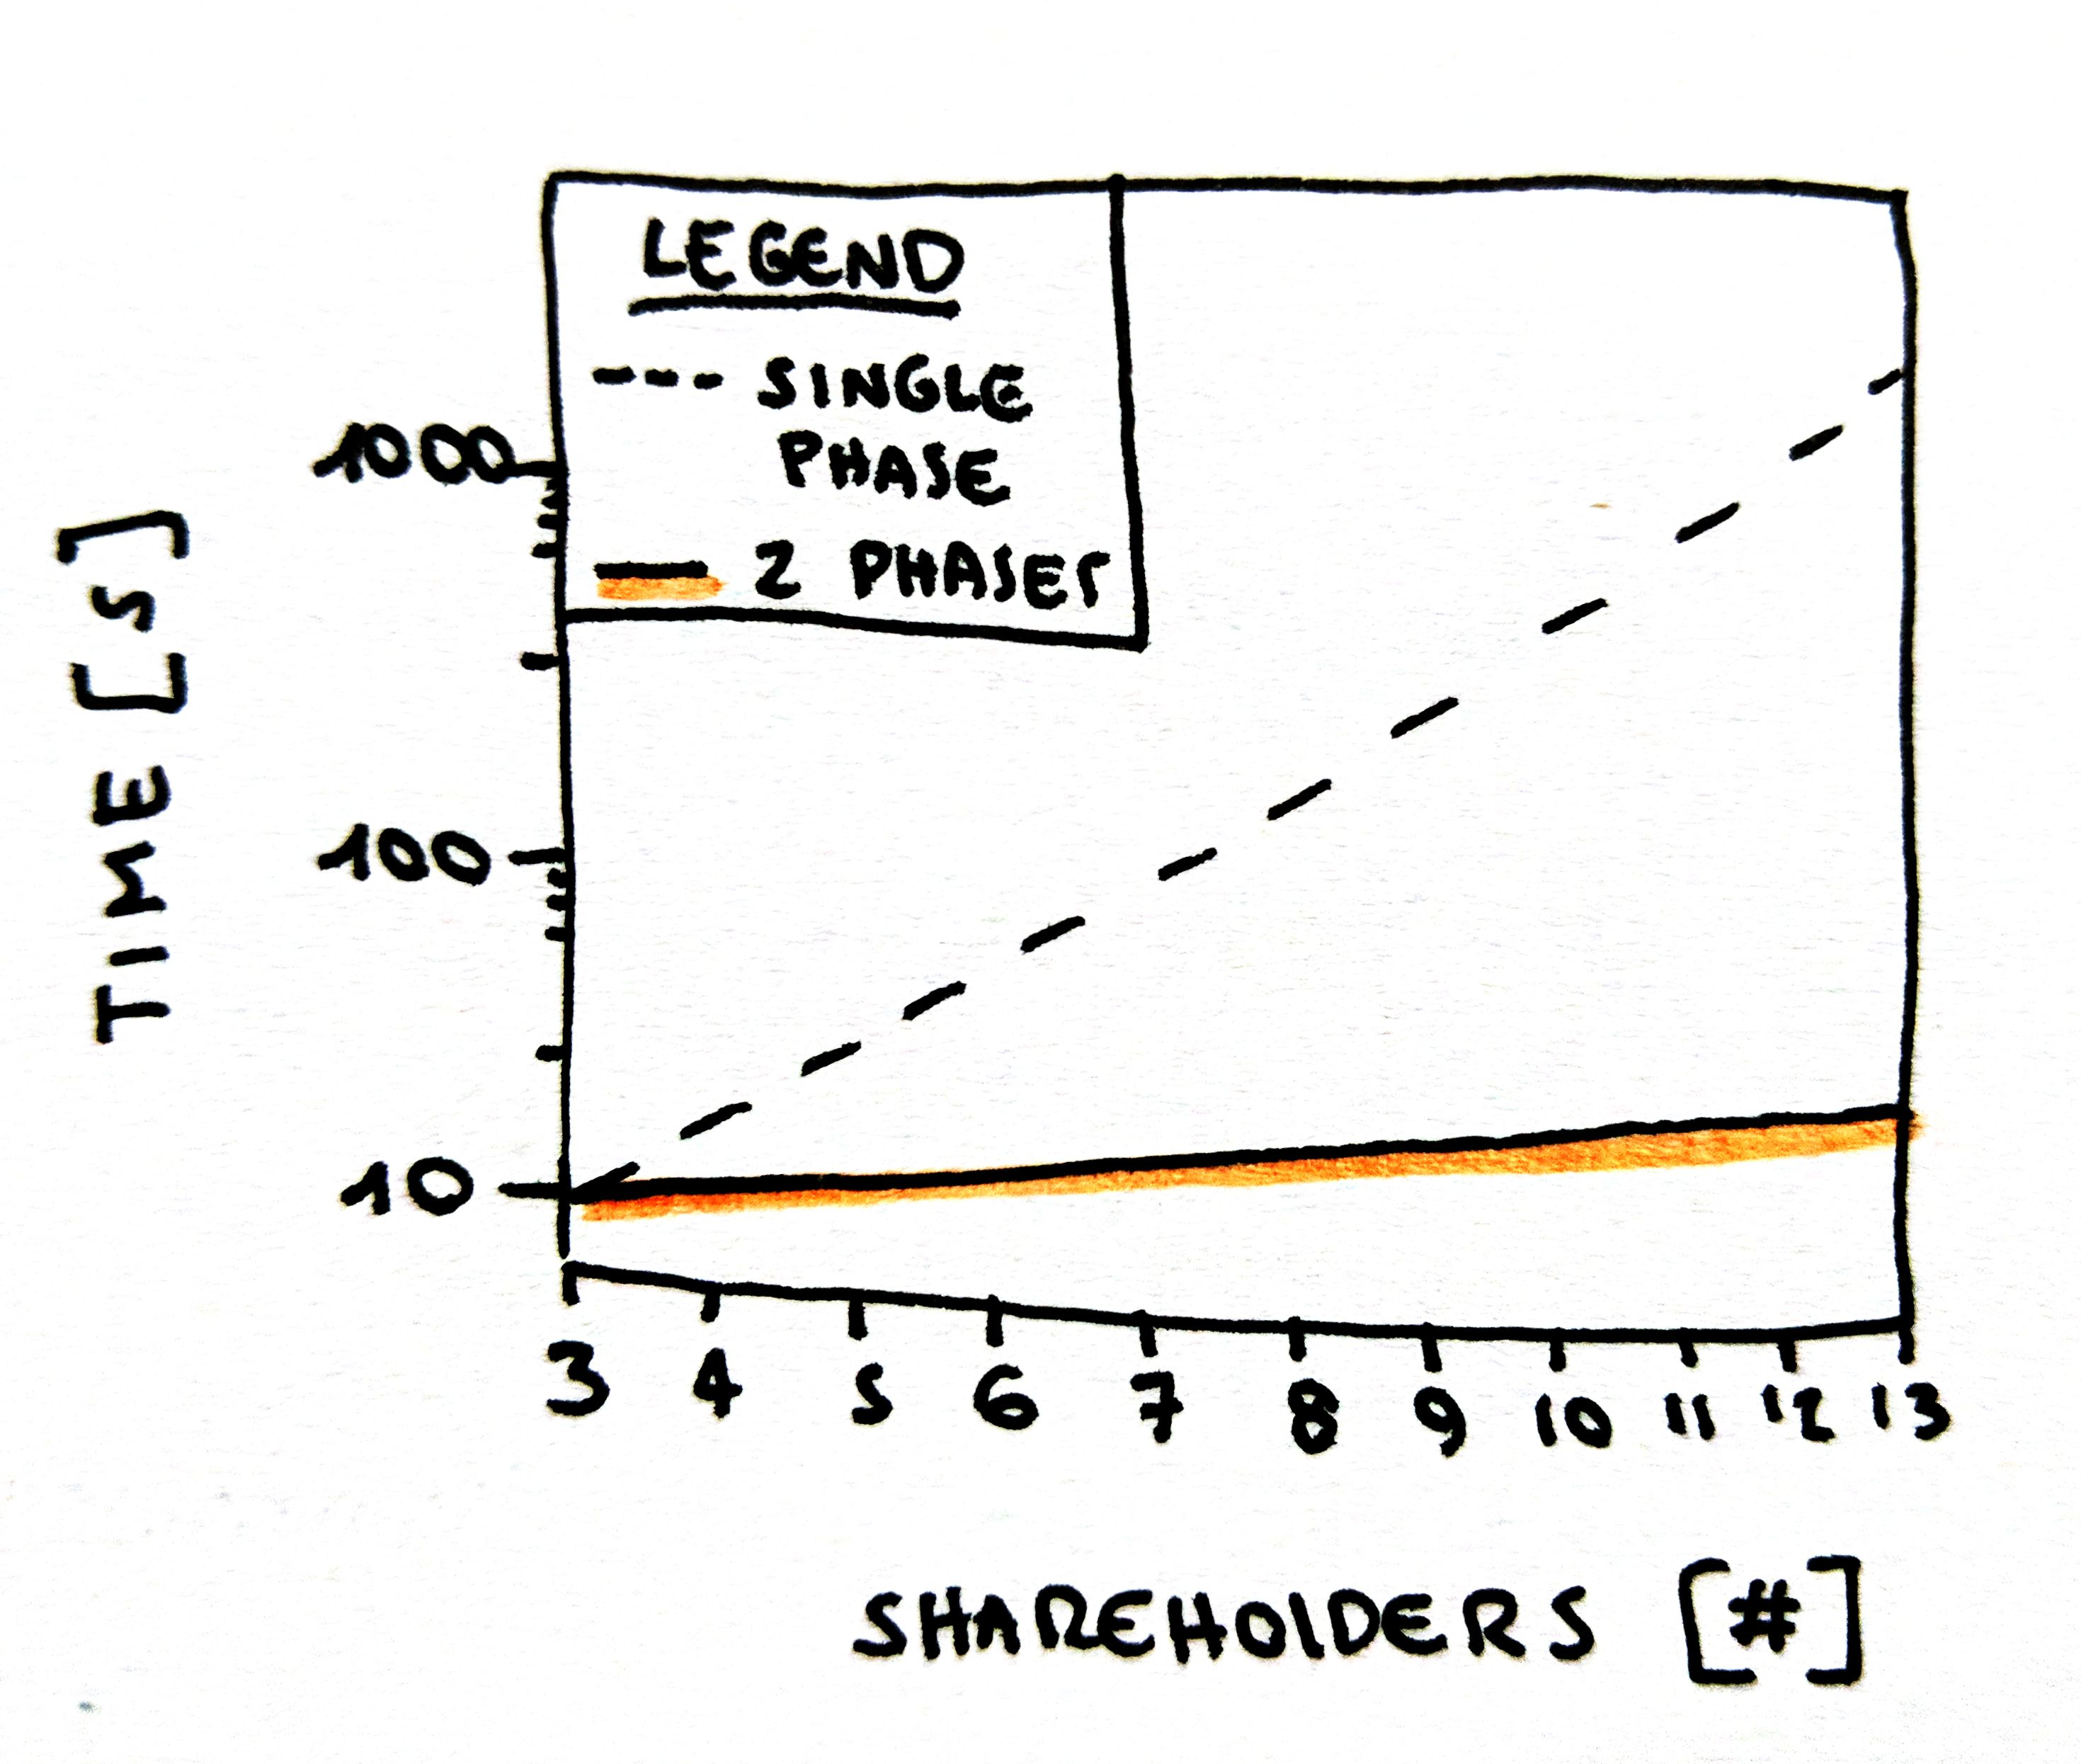
\includegraphics[width=0.7\columnwidth]{fig/mpc1vsmpc2}
	\caption{Time required by the two \shortname MPC protocols.}
	\label{fig:mpc1vsmpc2}
\end{figure}

\todo{move the second part of the (phase 1 and phase 2 here)}

\begin{itemize}
	\item description of the technologies used(formal validation of the state machine, gas and contract analyzer, algebraic vs arithmetic mpc protocols)
	\item introduction of the second mpc variant
	\item mpc comparative execution time demand
	\item monetary cost and space required by the two alternatives of the contract 
\end{itemize}



